%%% METHODOLOGY %%%
\clearpage
\section{Methodology}
This section defines the methodological plan followed in the thesis.
The process is organized into phases that move from requirements
analysis to design, implementation, and validation, while keeping an
iterative structure.

\subsection{Development process}
Since the expected outcome of the project is a software tool, the
development followed a conventional, iterative software engineering
process.

A simple and iterative development process was followed, allowing the
design to be refined as the project evolved.


The process was structured around a sequence of software engineering
phases, but it was not treated as a rigid waterfall. Each phase
provided context for the next one, while still allowing earlier
decisions to be revisited when implementation exposed practical
issues.

\subsubsection{Planned phases}
The proposed design methodology aims to transform the hypothesis of
this thesis into a working and validated exploration tool. According
to the evaluated state of the art, the development stages required to
accomplish the objectives and assess this hypothesis are summarized as
follows. Their role in the development process is introduced here,
while the resulting design decisions and implementation details are
described in the following chapters.

\begin{enumerate}
\item \textbf{Requirements analysis.} In this phase, the problem is
defined, the objectives are detailed, and the scope of the work is
established. Its main output is a functional specification that makes
the rest of the development less ambiguous. At this level, the tool is
required to:

\begin{figure}[htbp]
  \centering
  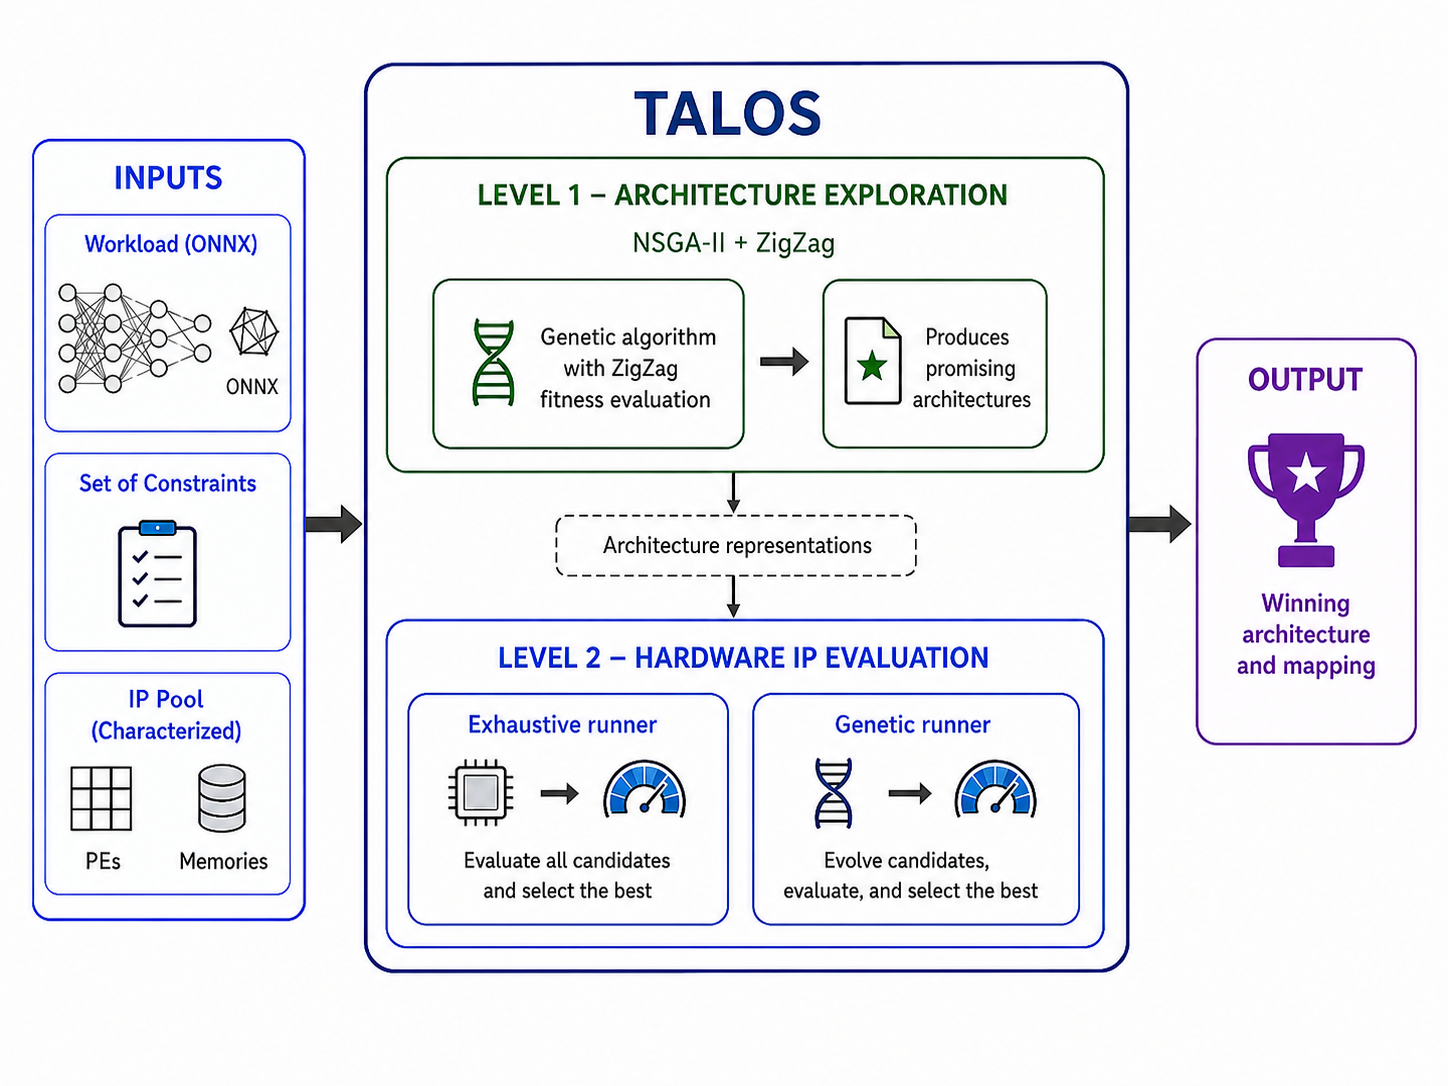
\includegraphics[width=\linewidth]{img/input_output.png}
  \caption{Talos input/output overview used to define the functional requirements.}
  \label{fig:talos-input-output}
\end{figure}

\begin{itemize}
\item accept a DNN workload in ONNX format;
\item load and validate a YAML pool of characterized processing
elements and memory IPs using a certain technology node;
\item generate and evaluate abstract accelerator architectures and
preserve the workload activity obtained for the selected candidates;
\item convert those candidates into Level~2 abstract components and
match them with compatible physical IP implementations;
\item reject implementations that cannot satisfy the required
capacity, bandwidth, throughput, frequency, or user constraints;
\item estimate workload latency, energy, average power, area, and
timing, while reporting the external DRAM contribution separately;
\item support configurable optimization objectives and both genetic
and exhaustive exploration; and
\item return feasible alternatives together with their metrics,
constraint status, and the mapping generated for each
selected architecture, instead of hiding the trade-offs behind one
design.
\end{itemize}

The ONNX workload is a central input of the flow. From the ONNX graph
and its tensor types, Talos infers the precision used for data
representation, generates the mapping of the workload on each
candidate architecture and estimates its cycles and memory accesses
in Level~1. The same precision is later used to select compatible
processing elements in Level~2.

The IP pool exposes the data that Level~2 requires to estimate PPA:
the area, timing, idle and active power of each block, together with
the operating point at which they were characterized. It also declares
the technology node, which is reused by the Level~1 calibration.

%figura here
The complete input and configuration requirements are specified in
Appendix~\ref{app:talos_requirements}.

\item \textbf{High-level design.} This phase turns the requirements
into a global structure. Its main output is the definition of the
two-level flow and the responsibilities of the main blocks of the
tool.

\item \textbf{Technical decisions and tooling selection.} This phase
selects the language, libraries, and external tools that will be
used. Its main output is a practical development stack that avoids
rebuilding existing solutions when they can be reused.

\item \textbf{Low-level design.} This phase defines the internal
representations and the interfaces between modules. Its main output
is a design with detailed enough to start implementation without
forcing every decision to be final from the beginning.

\item \textbf{Implementation.} This phase builds the modules
progressively and connects them into a first working flow. Its main
output is a prototype that can be executed and evaluated.

\item \textbf{Iterative refinement.} This phase revisits earlier
decisions when implementation exposes problems or better
alternatives. Its main output is a more coherent structure, obtained
by adjusting the design instead of treating the initial plan as fixed.

\item \textbf{Integration and validation.} This phase checks that the
different modules work together and that the result is aligned with
the original objectives. Its main output is a validated
implementation.
\item \textbf{HW Implementation.} This final phase corresponds to the finsl HW implementation of the obained solution using standard EDA tools for chi design (Cadence, Synompsis, Siemens).
\end{enumerate}

\subsection{Requirements analysis}
The first phase of the project consisted of defining the requirements
of the tool. At this stage, the objective was not yet to design
specific hardware instances, but to determine what kind of problem
the tool had to solve and which limitations of existing approaches it
should address.

From the beginning, one of the main requirements was not only to
provide a valid design space exploration flow for DNN accelerators,
but also to build the solution on top of a software architecture of
sufficient quality. Since this project is intended as a tool and not
just as a one-off prototype, the codebase had to be understandable,
maintainable, and easy to modify by a third party.

This was especially important in the context of a research project,
where requirements may evolve as new ideas appear. For that reason,
the solution had to avoid a monolithic structure and instead be
organized in a way that made future modifications possible without
having to redesign the whole system.

Another concern was to find a way to explore the vast solution space
in a reasonable time frame. DNN accelerator design involves many
parameters, including PE array dimensions, memory hierarchy,
dataflow, bandwidth, and hardware IP selection. Exploring all of them
directly at a detailed hardware level would make the problem
difficult to manage.

For that reason, an additional requirement was to separate the
exploration into two abstraction levels. The first level had to
remain lightweight enough to explore architectural candidates, while
the second level had to introduce hardware IP information only after
a candidate architecture had already been defined.

All these decisions influenced the next step, the high-level design
decisions.

\subsection{High-level design decisions}
Once the requirements were defined, the high-level design phase
started. In this stage, several possible approaches were considered
regarding how the tool should be structured and how existing tools
could be reused.

At this stage, the priority was to define a general architecture that
was clear and consistent. Rather than focusing on isolated
implementation details, the goal was to establish the main modules of
the tool, the responsibility of each one, and the way information
would flow between them.

One of the main design discussions was the approach to the
exploration of the space of solutions. After evaluating different
possibilities, the final decision was to adopt a two-level
architecture. The first level focuses on architectural exploration,
reducing the design space by exploring accelerator organizations,
memory hierarchies, dataflows, and PE array configurations. The
second level focuses on a more hardware-oriented evaluation of the
most promising candidates through abstract hardware IP models. Level
1 uses NSGA-II~\cite{nsga2} for architectural exploration. Level 2 can use NSGA-II
or exhaustive exploration; exhaustive exploration was added for
physical design spaces small enough to be evaluated completely.

This decision was relevant because it allowed the solution to
preserve flexibility while avoiding an early commitment to low-level
implementation details. It also provided a clearer separation between
architectural reasoning and hardware characterization, which became
one of the central ideas of the solution.

\subsection{Technical decisions and tooling selection}
Between the high-level design and the detailed design of each module,
several technical decisions were taken. These decisions were
necessary to make the proposed architecture implementable in practice.

At the software level, the tool was designed with special attention
to maintainability. The intention was not only to obtain a working
prototype, but to define an internal architecture that could be
understood and extended by another developer. This led to
prioritizing clear module boundaries, simple interfaces between
components, and a structure in which future modifications could be
introduced with limited impact on the rest of the system. In order to
keep access to the tool easy, Python was selected as the main
language of the tool.
However, there are some drawbacks, such as the execution speed.

A key decision was to use existing state-of-the-art tools as
conceptual and practical references for each level of the solution.
ZigZag was selected as the main reference for the first level because
it already provides architectural and mapping design space
exploration capabilities, including the study of memory hierarchies,
PE arrays, and dataflows. For the second level, the design was
influenced by the idea of using characterized hardware IP blocks,
similarly to generator-oriented approaches such as AutoDNNchip, but
without attempting to implement a complete RTL generation flow.

For NSGA-II, since it is a popular algorithm, different
implementations are available. In this case, \texttt{pymoo}~\cite{pymoo}
was chosen because it provides a practical implementation of
multi-objective evolutionary algorithms and allows the optimization
problem to be described with custom objective functions.

\subsection{Low-level design}
After defining the global structure of the tool, the low-level design
of each feature was addressed. In this phase, the focus shifted from
the abstract architecture of the project to the internal
representation of the design objects and the interfaces between
modules.

One of the most important tasks in this phase was defining how an
accelerator candidate should be represented inside the tool. Since
the tool had to support exploration and later evaluation, the
internal representation had to be expressive enough to capture
architectural parameters while remaining simple enough to be
manipulated and modified.

Another relevant part of this phase was the definition of the
interaction between both levels of the tool. The output of the first
level had to be structured in such a way that the second level could
reuse it without ambiguity. Therefore, the low-level design included
not only class and module definitions, but also the interfaces
between stages: which parameters are explored in the first level,
which are preserved for the second one, and how candidate designs are
passed from one stage to the next.

A major concern during this stage was keeping the software
architecture understandable. Rather than optimizing only for
short-term implementation speed, the design aimed to make the system
easier to extend and modify by third parties. This required defining
the responsibilities of each module carefully, limiting hidden
dependencies, and ensuring that each component had a clear role
inside the overall flow.

The Level 1 representation was defined as a discrete genome. Each
gene selects one value from a predefined set of architectural
options. In the current version, this genome contains seven genes: the
PE array dimensions, register-file size and bandwidth, global-buffer
size and bandwidth, and the PE-array dimensions served by the global
buffer. The latter parameter defines how the global buffer is shared
across the PE array, that is, along which spatial dimensions a single
global-buffer instance is accessible by multiple PEs. Depending on
this choice, the buffer may be shared by the entire array or replicated
across one of its dimensions. The external DRAM bandwidth was
intentionally left out of the genome and treated as a fixed platform
parameter, because the current model does not yet account for the
physical cost of the external memory interface.

The connection between Level 1 and Level 2 was defined through an
abstract accelerator representation. This representation contains
abstract components such as the PE array, register files, and global
buffer. These components express the requirements of the
architecture, while the second level is responsible for selecting
compatible IP blocks from the available IP pool. The abstract
representation is described in
Section~\ref{subsec:abstract_representation}, and the form of the IP
characterization that Level~2 matches against it, in
Section~\ref{subsec:ip_pool}; Appendix~\ref{app:ip_pools} reproduces
the pools used in the evaluation together with an annotated example
of one characterized IP. Figure~\ref{fig:abstract-arch} shows the
structure of this representation: a memory hierarchy feeding an array
of operational units, each with its local register files, in the same
terms used by ZigZag to describe an accelerator.

\begin{figure}[htbp]
  \centering
  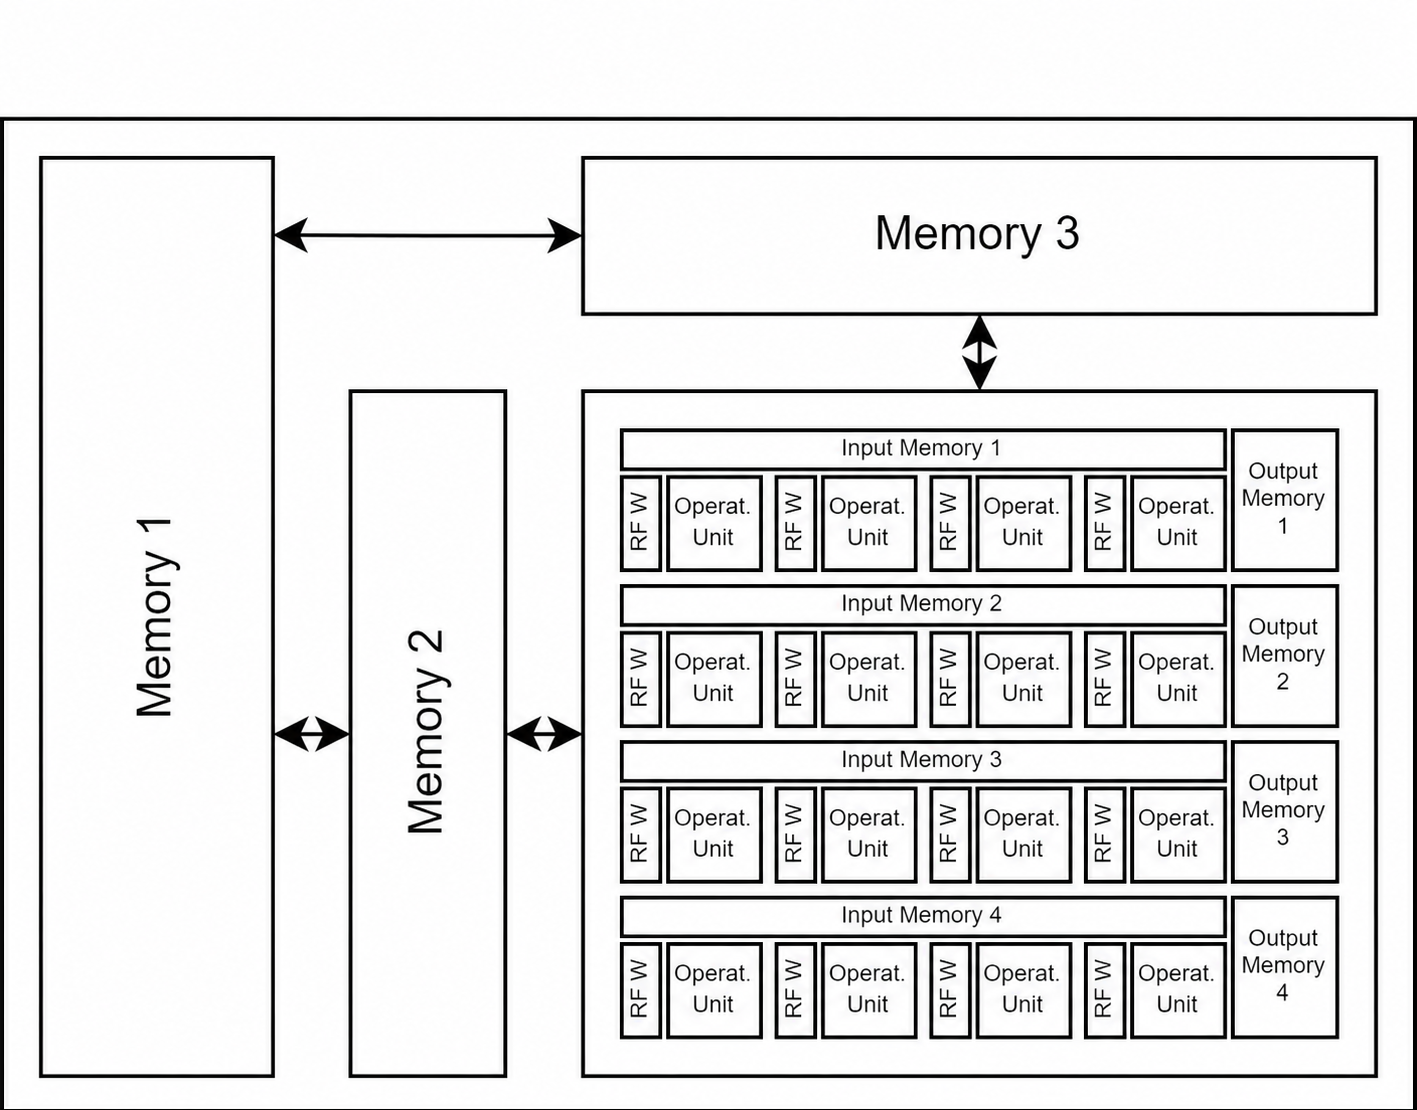
\includegraphics[width=0.85\linewidth]{img/abstract_arch.png}
  \caption{Abstract accelerator representation used to connect Level~1
  and Level~2. Adapted from the ZigZag hardware architecture
  documentation~\cite{zigzag_hardware_docs}.}
  \label{fig:abstract-arch}
\end{figure}

The Level 2 representation was therefore designed differently from
the first one. Instead of having a fixed genome, the Level 2 genome
is generated from the abstract accelerator itself. Each gene
corresponds to one abstract component and selects one compatible IP
implementation. This makes the second level flexible enough to handle
accelerator candidates with different component sets.

\subsection{Implementation}
Once the detailed design of the modules was sufficiently clear,
implementation began. This phase covered the actual construction of
the tool structure, the definition of the project modules, and the
first integration work with the selected exploration approach.

The implementation started from the basic software skeleton of the
project and progressively incorporated the main concepts defined in
the previous phases. In particular, effort was dedicated not only in
implementing functionality, but also in preserving the architectural
qualities defined during both design stages. This means keeping the
code organized around well-separated components and maintaining a
structure that would remain understandable as the project evolved.

At this stage, implementation was not a purely mechanical translation
of the design into code. On the contrary, coding exposed practical
issues that were not completely evident during design, such as how to
represent candidate architectures, how to connect the different
exploration stages, or how to preserve code clarity while introducing
new features. For that reason, implementation also acted as a source
of feedback for refining previous design decisions.

The implementation was built progressively. First, the architectural
genome (described in Subsection~\ref{subsec:genome}) and its decoder were implemented. Then, the generation of
ZigZag-compatible accelerator descriptions was added. After that, the
evaluator and objective extraction logic were introduced, allowing
raw evaluation results to be exposed as different optimization
objectives.

Once the first level was functional, the second level was
implemented. This included the abstract accelerator model, abstract
hardware components, IP block descriptions, IP pool loading,
compatibility checks, Level 2 genome generation, and the preliminary
PPA aggregation model.

\subsection{Iterative refinement}
Although the development process followed a clear sequence of phases,
it was intentionally iterative. In practice, the implementation of
each feature provided feedback that often required revisiting
previous design choices.

This happened, for example, when refining the architectural
representation of candidate accelerators, discussing how the design
variables should be encoded, or deciding how much information should
belong to the architectural exploration level and how much should be
deferred to the hardware-oriented evaluation level.

One concrete example of this refinement was the treatment of external
DRAM. Initially, DRAM bandwidth was considered as part of the
architectural genome. However, this allowed the optimizer to increase
off-chip bandwidth without paying any corresponding area or power
cost for the external interface. To avoid this unrealistic
optimization path, DRAM bandwidth was removed from the genome and
fixed as a platform parameter. The DRAM is still present in the
ZigZag memory hierarchy to model off-chip accesses, but it is not
considered part of the on-chip accelerator area or Level 2 IP
instantiation.

Another example was the introduction of the objective adapter.
Instead of hard-coding a single objective into the evaluator, this
component separates raw evaluation results from the objectives used
by the optimizer. This makes it easier to test different optimization
criteria without modifying the evaluator itself.

These iterations were not treated as deviations from the process, but
as a natural part of it. This was especially important in a
research-oriented software project such as this one, where some
design decisions could only be properly assessed after attempting a
concrete implementation.

As a result, the final development process was not a strictly linear
flow, but a controlled iteration between requirements, design, and
implementation until a coherent tool structure was obtained.

\subsection{Integration and validation}
The final part of the work integrated the different parts of the tool
and validated that the proposed approach was coherent with the
original objectives.

At the current stage of the project, this validation has focused
mainly on confirming that the methodology is viable: the hierarchical
structure has been defined, the modular architecture of the tool has
been established, ZigZag has been integrated as the exploration
engine for the first level, and the hardware IP characterization
approach for the second level has been implemented in a preliminary
form.

The validation was carried out through unit tests and smoke tests.
Unit tests were used to check individual modules, such as IP
validation, IP pool loading, compatibility checks, genome decoding,
implemented accelerator construction, and PPA evaluation. Smoke tests
were used to verify that a Level 1 architecture could be converted
into an abstract accelerator and then evaluated in Level 2 using an
example IP pool.

The validation of the physical estimates against synthesized designs
is presented in the Results chapter
(Table~\ref{tab:talos_estimation_validation}), once the hardware
implementation flow of the next subsection has been introduced.

\subsection{HW Implementation}
\label{subsec:hw_implementation}
The last phase of the methodology takes the configuration selected by
Talos to a hardware implementation with standard EDA tools. The
proposed design flow has three steps. First, the selected
implementation is assembled in SystemVerilog by composing the same RTL
blocks that were characterized for the IP pool: the number of
instances, the array dimensions, the interfaces and the precisions are
fixed through parameterized top-level wrappers, so no new datapath RTL
is written for a given candidate. Second, the design is elaborated and
synthesized with Cadence Genus against the standard-cell library of the
target technology, and area, timing and power are extracted from the
mapped netlist. Third, when a physical result is required, the netlist
can be taken through placement and routing with Cadence Innovus and,
if a test chip is intended, through the sign-off steps of the
corresponding PDK. The technologies available at the UAB through its
EDA and foundry-access agreements are the natural targets of this
flow; in this thesis it was applied up to the synthesis step, using
the TSMC 65~nm low-power library, which is also the step used to
build the IP pool.
\todo[inline]{PENDIENTE: confirmar y listar las tecnologías/PDKs y
herramientas disponibles en la UAB que se quieren nombrar aquí (p.ej.
TSMC 65~nm LP vía Europractice, otros nodos, Innovus para P\&R).}

Table~\ref{tab:ip_pool_sources} lists the origin of the RTL blocks
behind the pool entries reproduced in Appendix~\ref{app:ip_pools}. The
processing elements were taken from open-source accelerator designs or
written as simple MACs, the register files are BaseJump STL memories
and the global buffers are OpenEye single-port RAMs. The requirements
that a pool entry must satisfy (fields, units and operating point) are
given in Appendix~\ref{app:talos_requirements}; the characterization
described next produces exactly those fields.
\todo[inline]{PENDIENTE: añadir referencias o URLs de los repositorios
de origen del RTL de terceros (tiny-XPU, Gemmini, OpenEye, BaseJump
STL, FPnew, PE de Alibaba, PE TMS4517) en la
Tabla~\ref{tab:ip_pool_sources} y en la bibliografía.}

\begin{table}[htbp]
\centering
\caption{Origin of the RTL blocks characterized for the IP pools.}
\label{tab:ip_pool_sources}
\footnotesize
\setlength{\tabcolsep}{4pt}
\renewcommand{\arraystretch}{1.15}
\begin{tabular}{@{}>{\raggedright\arraybackslash}p{4.4cm}>{\raggedright\arraybackslash}p{3.3cm}>{\raggedright\arraybackslash}p{6.0cm}@{}}
\hline
\textbf{Pool entries} & \textbf{Source RTL} & \textbf{Notes} \\
\hline
\texttt{pe\_sauria}, \texttt{pe\_sauria\_int16},
\texttt{pe\_sauria\_fp16} &
SAURIA systolic PE~\cite{sauria2023} &
INT8, INT16 and FP16 variants; the FP16 one wraps a modified FPnew
FMA \\
\texttt{pe\_fpnew\_fp16\_fma} &
FPnew FMA unit &
Bare FP16 FMA without the systolic wrapper; used by the synthesized
FP16 accelerator \\
\texttt{pe\_gemmini\_like},
\texttt{pe\_gemmini\_like\_int16} &
Gemmini-inspired PE &
INT8 with selectable OS/WS dataflow; the INT16 variant is fixed to OS \\
\texttt{pe\_tiny\_xpu}, \texttt{pe\_tiny\_xpu\_int16} &
tiny-XPU PE &
Weight-stationary MAC; used by the synthesized INT16 accelerators \\
\texttt{pe\_alibaba\_int8} &
Alibaba systolic PE &
Ping-pong weight registers, four pipeline stages \\
\texttt{pe\_tms4517\_simple} &
TMS4517 systolic PE &
Unsigned operands, single stage \\
\texttt{pe\_simple\_mac} &
Own reference MAC &
Signed INT8 MAC without systolic logic; used by the synthesized INT8
accelerator \\
\texttt{pe\_openeye\_\allowbreak composite\_int8} &
OpenEye PE &
Composite sparse PE with local scratchpads (declared through
\texttt{included\_rfs}) \\
\texttt{mem\_bsg\_1rw\_*}, \texttt{mem\_bsg\_1r1w\_*} (12) &
BaseJump STL \texttt{bsg\_mem} &
1RW and 1R1W register files, 8 words of 8 to 256 bits, synthesizable
(non-macro) variants \\
\texttt{mem\_openeye\_sp\_*} (3) &
OpenEye \texttt{RAM\_SP} &
Single-port global buffers, 128 words of 64, 256 and 1024 bits \\
\hline
\end{tabular}
\end{table}

The pools used in this work are an example. Talos does not
include a characterized library, before running Level~2, the user has
to provide a pool for the target technology. The rest of this
subsection describes how the pools of this work were built, so that
the process can serve as a guide.

The blocks were taken from open-source accelerator designs. Some were
used as they are. Others were modified to obtain a variant that was
not available, such as the INT16 versions of some PEs, or written as
simple reference blocks, such as \texttt{pe\_simple\_mac}. Each block
was wrapped in a small SystemVerilog top level with a single clock, an
active-low reset and the parameters of the variant (precision, depth
or width). Each variant was then synthesized separately, and its
characterization was taken directly from the Genus reports.

All blocks were synthesized with Cadence Genus 23.15 using the TSMC
65~nm low-power 9-track standard-cell library (\texttt{tcbn65lptc})
at the nominal NCCOM/TT corner (1.2~V, 25~$^\circ$C), with a 5~ns
clock (200~MHz), input and output delays of a tenth of the period and
a fixed output load. Memories were synthesized from RTL into standard
cells rather than treated as opaque SRAM macros, and the external DRAM
and its PHY were excluded from the accelerator silicon boundary. Area
was read from the area report as mapped cell area, without wires or
placement effects. The critical path was read from the timing report,
and the maximum frequency was derived from its
slack\footnote{$f_{\max} = 1000 / (T_{\mathrm{clk}} - \mathrm{slack})$
in MHz, with $T_{\mathrm{clk}}$ and the slack in ns. Since the designs
were constrained at 5~ns, blocks with positive slack report an
$f_{\max}$ above 200~MHz.}.

Idle and active power were obtained with two vectorless power
estimations of Genus on the same mapped netlist. In the idle scenario
the reset is deasserted, the clock runs and all data and control
inputs are held constant: the block is clocked but performs no
operation or access. In the active scenario the data inputs toggle
randomly and the control inputs are set so that the block performs
one operation or access per cycle\footnote{Random data assume a
toggle probability of 0.5 and 0.5 transitions per cycle per bit, that
is, 0.1 toggles/ns at 200~MHz; control inputs that alternate every
cycle toggle at 0.2 toggles/ns; constant controls do not toggle. For
memories, the active value stored in the pool corresponds to a mixed
read/write scenario.}. Vectorless estimates have no temporal
correlation between signals and no activity from a real stimulus, so
they are less accurate than SAIF- or VCD-based analysis. They were
chosen because they apply the same assumptions to every block, which
is what Level~2 needs to compare implementations. The same script was
used, with the accelerator top level as the target, for the four
synthesized configurations validated in
Section~\ref{sec:synthesis_validation}, whose reports are reproduced
in Appendix~\ref{app:synthesis_reports}.

Finally, the values of the reports were transcribed by hand into the
pool files described in Appendix~\ref{app:talos_requirements}: area in
mm$^2$, delay and maximum frequency, idle and active power with their
operating point, and the metadata that synthesis does not produce,
such as MACs per cycle, pipeline latency, the register files included
in a composite PE or the numerical format. This process is manual but
repetitive. Since the wrappers, the synthesis script and the YAML
format are fixed, it can be automated with a script that iterates over
the variants, runs the synthesis and emits the pool entries. This is
left as future work.

\subsection{Summary of the chapter}
The development milestones introduced in the Subsection~\ref{subsec:milestones} provide a
direct way of assessing the resulting framework.

Milestone~\ref{milestone:m1} was fulfilled through the definition of the
two-level methodology. Architectural exploration is performed in
Level~1 without selecting physical IPs, while Level~2 introduces the
technology-dependent implementations. The abstract accelerator
representation connects both levels without removing this separation.

Milestone~\ref{milestone:m2} was fulfilled through the Level~1 genome,
NSGA-II exploration, using ZigZag which generates mappings for the
candidate architectures and evaluates them according to the selected
objectives. Together, these elements
automatically generate candidate architectures, evaluate their
mapping, energy, latency, and area-related cost, and preserve the
selected alternatives for the second level.

Finally, the methodology and its implementation were validated with
four workload configurations and characterized INT8, INT16, and FP16
hardware pools. The selected implementations were also compared with
published accelerators and synthesized designs. The complete
experimental results are presented in the Results chapter. These
results show that the framework can reduce and rank the design space
using physical IP information. They also delimit the scope of this
milestone: the model supports architectural selection, but the final
candidates still require conventional synthesis for accurate physical
results.

Therefore, the milestones established in the Introduction were
covered within the scope of the thesis, from the definition of the
hierarchical methodology to its experimental validation as a working
software prototype.
